%%%%%%%%%%%%%%%%%%%%%%%%%%%%%%%%%%%%%%%%%%%%%%%%%%%%%%%%%%%%%%%%%%%%%%%%%%%%%%
% Continuum Mechanics Coursenotes
%
% $Id$
%%%%%%%%%%%%%%%%%%%%%%%%%%%%%%%%%%%%%%%%%%%%%%%%%%%%%%%%%%%%%%%%%%%%%%%%%%%%%%
\documentclass[a4paper,11pt]		{report}
\usepackage{amsmath,amssymb,amsxtra,bm,natbib,graphicx,epic,eepic,textcomp}
%\usepackage[all,import]{xy}

\graphicspath{{./Figs/}} 

\setlength{\textheight}			{245mm}
\setlength{\textwidth}			{165mm}
\setlength{\topmargin}			{-5mm}
\setlength{\headsep}			{0mm}
\setlength{\oddsidemargin}		{0mm}
\setlength{\parsep}                     {0mm}

\renewcommand{\baselinestretch}		{1.00}

\input{hmb.mac}

%%%%%%%%%%%%%%%%%%%%%%%%%%%%%%%%%%%%%%%%%%%%%%%%%%%%%%%%%%%%%%%%%%%%%%%%%%%%%%
\begin{document}

\begin{titlepage}
\biomedsubject{421-286}{Bioengineering Systems 2}{2006}

\vspace*{15em}

\begin{center}
{\huge
An Introduction to Continuum Mechanics\\[5pt]
for Biomedical Applications
}

\vspace*{15em}

{\Large Hugh M Blackburn}

\end{center}

\end{titlepage}

%\maketitle


%%%%%%%%%%%%%%%%%%%%%%%%%%%%%%%%%%%%%%%%%%%%%%%%%%%%%%%%%%%%%%%%%%%%%%%%%%%%%%
\part{Continuum mechanics}
%%%%%%%%%%%%%%%%%%%%%%%%%%%%%%%%%%%%%%%%%%%%%%%%%%%%%%%%%%%%%%%%%%%%%%%%%%%%%%





%#############################################################################
\chapter{Continua}
\label{ch.cont}

At biological length scales it often becomes difficult to ignore the
discrete nature of the materials involved. However, in order to make
progress in analysing large-scale mechanical effects, \eg on the
length scale of the human body, or of the larger arteries, we usually
need to assume the materials involved are continua. The three
fundamental kinds of continua are solids, liquids and gases. Sometimes
we group liquids and gases together as fluids, on the basis of the
similarity of their mechanical behaviours.

%%%%%%%%%%%%%%%%%%%%%%%%%%%%%%%%%%%%%%%%%%%%%%%%%%%%%%%%%%%%%%%%%%%%%%%%%%%%%%
\section{Basic properties of solids and fluids}

The basic distinction between solids and fluids is that solids in
equilibrium (\ie at rest) can resist shear stress, whereas fluids,
both gases and liquids, cannot. If fluids are subjected to a shear
stress (\ie a tangential stress), they deform continuously in time and
space until the shear stress reaches zero, as shown in
figure~\ref{fig.def}.

\begin{figure}
\begin{center}
\includegraphics[width=0.6\textwidth]{Shames-1.1.eps}
\end{center}
\caption{The most basic difference between solids and fluids is that
  when placed under shear, solids reach a fixed deformation whereas
  fluids deform continuously.
  \citep[From][]{shames62}}
\label{fig.def}
\end{figure}

The basic distinction between a liquid and a gas is that liquids have
a distinct surface, whereas gases do not. If placed inside a
container, a gas expands to fill it (and if the container is not
closed, it will expand continuously), while a liquid will fill only a
fixed volume of the container, and be separated from the surroundings
by the walls of the container and a `free surface', as illustrated in
figure~\ref{fig.slg}.

\begin{figure}
\begin{center}
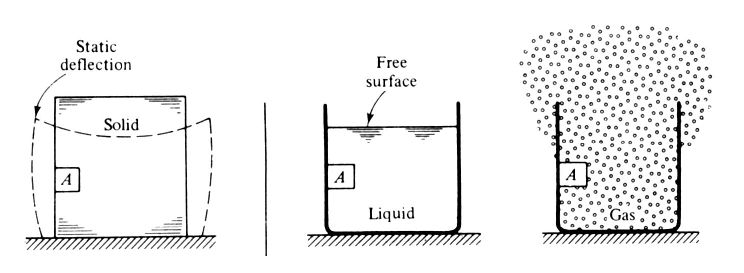
\includegraphics[width=0.6\textwidth]{White-1.1.eps}
\end{center}
\caption{The distinct behaviours of solids, liquids and
gases. \citep[From][]{white86}}
\label{fig.slg}
\end{figure}

A related property is that gases are much more readily compressed from
one volume to to a smaller one by an increase in pressure than are
liquids: a gas is much more elastic, and we say that it is more
compressible. By comparison to gases at typical temperatures and
pressures, liquids are practically incompressible. On the other hand,
in typical biomedical situations\,---\,and in a large number of
engineering applications\,---\,the amount of pressure change in a gas
compared to the background (atmospheric) pressure is comparatively
small, hence compression is comparatively weak, and gases may often
also be approximated as flowing incompressibly.

Of course, it is generally possible to convert a solid to a liquid and
then a gas by application of heat. We will not be considering these
phase change effects, but ultimately it is the relative amount of
internal thermal energy, reflected in the degree of relative motion
between molecules, that provides the difference in mechanical
behaviours between solid, liquid and gas phases of the same
material. The mechanical properties of solids, liquids and gases are
directly related to their molecular structure and the forces between
molecules. As a broad statement, these are related to the
characteristic distance between the molecules of a particular
material, and on how the forces between the molecules varies with
distance. At small distances (of order $10^{-10}$m), there is a strong
force of quantum origin between the molecules, related to the
possibility of exchange of electron shells \ie the formation of a
chemical bond. In the case that a chemical bond will not be formed,
the force is repulsive and falls off very rapidly as the distance
between the molecules increases. At larger distances, a weakly
attractive force (van der Waal's force) becomes dominant. The
combination of these two effects gives rise to the functional shape
seen in figure~\ref{fig.lj}. The equilibrium distance $d_0$ is of
order $4\times10^{-10}$m for most simple molecules.

\begin{figure}
\begin{center}
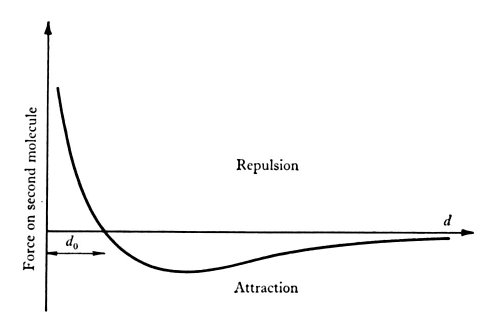
\includegraphics[width=0.45\textwidth]{Bat-1.1.1.eps}
\end{center}
\caption{Force exerted by one (uncharged) simple molecule on another
  as a function of the distance between them. The equilibrium distance
  is $d_0$. \citep[From][]{bat67}}
\label{fig.lj}
\end{figure}

At room temperature and pressure the average distance between the
centres of adjoining molecules is of order $10d_0$ for gases, and of
order $d_0$ for liquids and solids. The properties of gases can to
quite a large extent be analysed using the statistics of random
collisions between isolated molecules. In a solid, the molecules are
held in a more-or-less fixed orientation relative to one another (\eg
in a perfect crystal, the orientation is completely periodic in all
directions). There is still some random thermally driven vibration of
positions of individual molecules. In a liquid, the situation is more
complicated, because the state is neither completely ordered nor
completely random. It is now becoming possible to compute or simulate
the behaviour of liquids from first principles, but the total number
of molecules involved in a single simulation is far too small to be
able to deal with `large-scale' problems (lengths say of order a
millimetre and above). The molecular properties of solid, liquid and
gases phases are summarised in table~\ref{tab.bat1}.

\begin{table}
\begin{center}
\begin{tabular}{cp{25mm}p{35mm}p{28mm}p{30mm} }
\hline
Phase & 
\centering{Intermolecular forces} & 
\centering{Ratio of random thermal movement of molecules to $d_0$} &
\centering{Molecular arrangement} &
Type of statistics needed \\[5pt]
solid & \centering{strong} & 
\centering{$\ll1$} & \centering{ordered} & \multicolumn{1}{c}{quantum} \\
liquid & \centering{medium} & 
\centering{${\cal O}(1)$} & \centering{partially ordered} & \multicolumn{1}{c}{quantum + classical} \\
gas & \centering{weak} & \centering{$\gg1$} & \centering{disordered} &
\multicolumn{1}{c}{classical} \\ \hline
\end{tabular}
\end{center}
\caption{The characteristics of solid, liquid and gas
  phases. \citep[From][]{bat67}}
\label{tab.bat1}
\end{table}

We will return to describing the mechanical properties of solids and
fluids in chapter~\ref{ch.constit}.

%%%%%%%%%%%%%%%%%%%%%%%%%%%%%%%%%%%%%%%%%%%%%%%%%%%%%%%%%%%%%%%%%%%%%%%%%%%%%%
\section{The continuum hypothesis}

Whether or not we can consider a material as a continuum depends on
the length scales at which we examine it, and if we can form a stable
statistical description or not at the length scales of interest.
Imagine measuring say the density of a gas by counting the number of
molecules within a certain volume, then dividing by the volume to
estimate density. Clearly if the volume is extremely small, say only
large enough to contain a few molecules at a time, then the density
will fluctuate as molecules enter and leave the volume under the
influence of Brownian motion. As we increase the volume, we will be
averaging over more and more molecules, and the estimate of density
will reach a stable value. This situation is illustrated in
figure~\ref{fig.bat2}, where the size of the volume at which this
stable local estimate is reached is labelled $\delta V^\ast$. If,
however, we keep increasing the measurement volume, then we could
start to move away from this local value because the local average
density (the `continuum value') varies from place to place, and our
averaging starts to reflect this.

\begin{figure}
\begin{center}
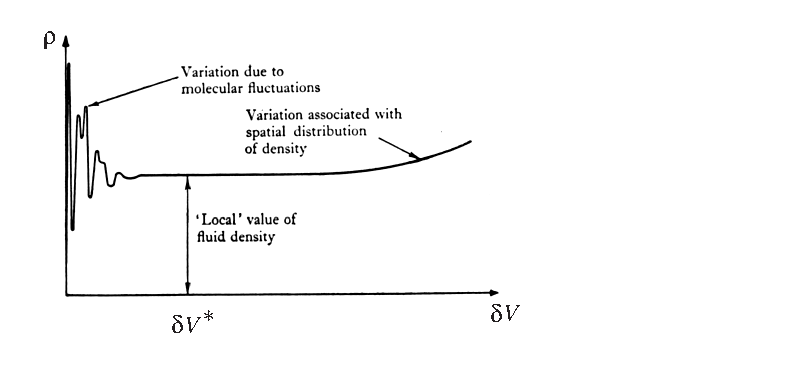
\includegraphics[bb=10 15 245 167,clip,width=0.45\textwidth]{Bat-1.2.1-mod.eps}
\end{center}
\caption{Illustration of the effect of increasing the measurement
  volume $\delta V$ on the estimate of density,
  $\rho$. \citep[After][]{bat67}}
\label{fig.bat2}
\end{figure}

The volume $\delta V^\ast$ is very small: its value is of order
$10^{-9}$mm$^3$ (\ie a cube $10^{-3}$mm on a side) for all liquids and
gases at atmospheric pressure. A cube of air this size contains about
$3\times10^{7}$ molecules at room temperature and pressure. By
definition then, our study of continuum mechanics deals with matter at
length scales larger than approximately one-thousandth of a
millimetre, or one micron. This is generally small enough in
comparison to the length scales dealt with that the density (or any
other measure) can be thought of as a point function, and the material
properties to vary continually in space. We call such a material a
continuum, and can analyse its motion using differential calculus.

%%%%%%%%%%%%%%%%%%%%%%%%%%%%%%%%%%%%%%%%%%%%%%%%%%%%%%%%%%%%%%%%%%%%%%%%%%%%%%
\section{Coordinate systems}

When dealing with problems of continuum mechanics, we are always faced
with the need to describe field variables (concentrations,
displacements, velocities, accelerations, stresses and strains) which
vary in space. We are used to thinking in terms of a Cartesian spatial
coordinate system, with three axes which are rectilinear and
orthogonal, and with expressing the spatial dependence of variables in
terms of these three coordinates (usually taken as $x$, $y$ and $z$,
or equivalently $x_1$, $x_2$ and $x_3$). From the point of view of
introducing the concepts involved, this is usually the most
straightforward option. However, if the problem has some special
symmetry, then we might want to work in some other coordinate system
(\eg cylindrical or spherical, where again the directions are locally
orthogonal, but the axes are not rectilinear), or even in one that
gives up orthogonality of coordinate directions.

However, the natural language of continuum mechanics deals in vectors
and tensor quantities. (A tensor is a higher-dimensional generalisation
of a vector, which in turn is a first-order tensor.) The advantages of
this are two-fold. First, the statements are much more concise in
vector form. Second, because vectors and tensors have a physical
meaning (in the sense that a vector always possesses the same
direction and length, regardless of the coordinate system in which it
may be described), the descriptions in terms of vector notation are
coordinate-free, \ie the same in any system of coordinates. A related
effect is that the physical meaning of an expression written in vector
notation is readily identified.

As befits an Introduction to the area, we will usually work in a
Cartesian coordinate system, and not rely heavily on vector and tensor
notation, or vector calculus. When appropriate, and it ought not stand
in the way of interpretation, we will use simple vector notation. For
example we will often take $\bm{x}$ as a shorthand for the vector $(x,
y, z)$, and $\bm{u}$ as a shorthand for the vector $(u, v,
w)$. Another notation we will make some use of is the gradient
operator $\bm{\nabla}$, which has the Cartesian-coordinate expression
\[
\bm{\nabla}\equiv\bm{i}\frac{\partial}{\partial x}+
\bm{j}\frac{\partial}{\partial y}+\bm{k}\frac{\partial}{\partial z},
\]
where $\bm{i}$, $\bm{j}$ and $\bm{k}$ are the unit vectors parallel
with the $x$, $y$, and $z$ axes respectively.  Two texts which give a
particularly clear outline of vector and tensor methods as applied to
continuum mechanics are \citet{aris62} and \citet{dan92}.

%%%%%%%%%%%%%%%%%%%%%%%%%%%%%%%%%%%%%%%%%%%%%%%%%%%%%%%%%%%%%%%%%%%%%%%%%%%%%%
\section{The idea of stress in a continuum}

Two fundamental considerations in the mechanics of continua are how
forces are transmitted within them, and how they respond by
deformation. We have already used the term stress; now we will begin
to study this idea more closely. Stress produces deformation and
failure in solids, and motion of fluids. The material in this and the
following section are discussed in much greater depth by
\citet{fung69} and \citet{aris62}.

%=============================================================================
\subsection{Body forces}

In continuum mechanics, we are generally concerned with two kinds of
forces that can be exerted on a material region: surface forces (as
the name implies, exterted over a surface) and body forces, or forces
that are distributed through the volume. We will deal with surface
forces in the following section, but first we will briefly consider
body forces. The one with which we are most familiar is that of
gravitational attraction, and that will generally serve as the example
used, simply because of its universality and importance.  Consider a
volume of fluid $\Delta V=\Delta x\Delta y\Delta z$, with density
$\rho$. Then the value of the body force per unit volume is $\rho\mathbf{g}$,
where $\mathbf{g}$ is the vector of gravitational acceleration; the total
force experienced by the volume is $\rho\mathbf{g}\Delta V=\mathbf{g}\Delta m$.

Other kinds of body forces, such as magnetic or electrodynamic forces,
may be important in specific applications. If we are carrying out a
solution in an accelerating frame of reference, then it often is
easiest to replace or augment gravitational attraction with the frame
acceleration.

%=============================================================================
\subsection{The traction vector}

Suppose we have a continuum occupying region $B$, and within it, a
closed surface $S$, as shown in figure~\ref{fig.tract}. On some
elemental sub-surface $\Delta S$, with unit outward normal vector
$\bm{n}$, a force $\Delta\bm{F}$ is exerted on the material inside $S$
by that outside. We assume that as the area $\Delta S\to0$, the ratio
$\Delta\bm{F}/\Delta S$ reaches a limit $\cd\bm{F}/\cd S$ and that the
moment of the force acting on the surface $\Delta S$ about any point
within $\Delta S$ vanishes in the limit.  The limiting vector 
\begin{equation}
\stackrel{\bm{n}}{\bm{T}}=\frac{\cd\bm{F}}{\cd S}
\end{equation}
is called the traction, or stress vector, and represents the force per
unit area acting on the surface.  The idea that the material outside a
surface can be considered to act on the material inside through
tractions in this way was formalised by Euler and Cauchy.  Note the
superscript $\bm{n}$: this is used to indicate that the traction
vector depends on the local orientation of the unit outward normal,
$\bm{n}$, \emph{as well as} the location of $\cd S$. Locally, the
traction that the material inside $S$ exerts on the material outside
$\cd S$ is equal and opposite, \ie $-\stackrel{\bm{n}}{\bm{T}}$; this
is linked directly to the fact that the unit normal is reversed (or,
equivalently, Newton's First Law), but the dependence of $\bm{T}$ on
$\bm{n}$ is more far-reaching than this.

\begin{figure}
\begin{center}
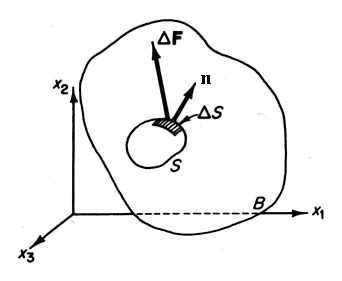
\includegraphics[width=0.30\textwidth]{Fung-3.1.eps}
\end{center}
\caption{The idea of a traction on a surface, leading to the
  definition of stress. \citep[After][]{fung69}}
\label{fig.tract}
\end{figure}

%=============================================================================
\subsection{Stress and stess components}

\begin{figure}
\begin{center}
%\begin{tabular}{cccc}
%\raisebox{12ex}{(\textit{a})} &
%\raisebox{2ex}{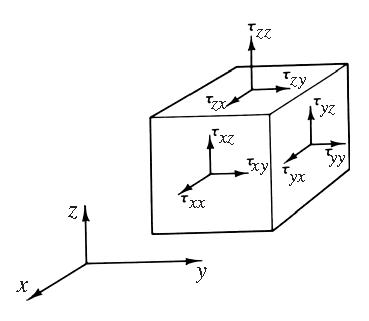
\includegraphics[width=0.35\textwidth]{Fung-3.2.eps}} &
%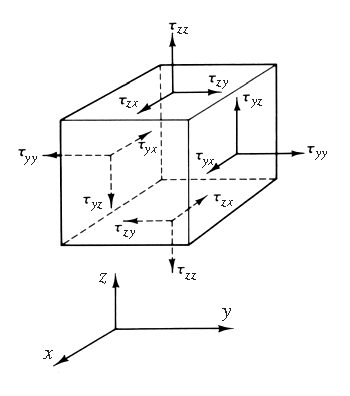
\includegraphics[width=0.30\textwidth]{Fung-3.3.eps} &
%\raisebox{12ex}{(\textit{b})}
%\end{tabular}
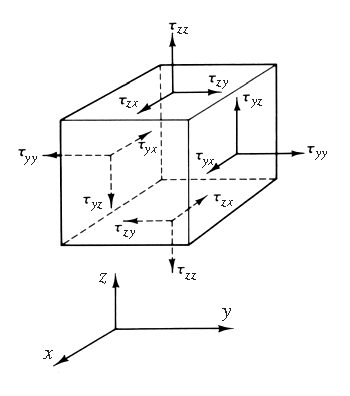
\includegraphics[width=0.33\textwidth]{Fung-3.3.eps}
\end{center}
\caption{Notation of stress components at a point in Cartesian
  space. Components $\tau_{ij}$ are indexed first ($i$) by the
  direction of the outward normal of the relevant face, and secondly
  ($j$) by the direction in which the component points.  Note that
  when the orientations of the faces are reversed, so are the
  components, although their names stay the same.}
\label{fig.stress}
\end{figure}

To simplify matters, first consider a case where the surface $\Delta
S_k$, $k=x$, $y$, or $z$, is parallel with one of the coordinate
planes, \ie where the unit normal $\bm{n}$ points in the same
direction as one of the coordinate axes.  Let the corresponding
traction on $\Delta S_k$ be $\stackrel{k}{\bm{T}}$, with three
components $\stackrel{k}{T}_x$, $\stackrel{k}{T}_y$,
$\stackrel{k}{T}_z$. Then in this special case the traction components
are the same as those of the underlying \emph{stress tensor},
$\bm{\tau}$, with
\begin{equation}
\stackrel{k}{T}_x=\tau_{kx}, \qquad
\stackrel{k}{T}_y=\tau_{ky}, \qquad
\stackrel{k}{T}_z=\tau_{kz}.
\end{equation}
For each direction $k=x$, $y$, $z$, there will be three such
components, and we can write them in a square matrix array
\begin{center}
\begin{tabular}{cccc}
& \multicolumn{3}{c}{Components of stress tractions}\\
& \hspace*{3ex}$x$\hspace*{2ex}&\hspace*{2ex}$y$\hspace*{2ex}&\hspace*{2ex}$z$\hspace*{3ex}\\
Surface normal points along $x$ &\hspace*{3ex}$\tau_{xx}$\hspace*{2ex}&\hspace*{2ex}$\tau_{xy}$\hspace*{2ex}&\hspace*{2ex}
$\tau_{xz}$\hspace*{3ex}\\
Surface normal points along $y$ &\hspace*{3ex}$\tau_{yx}$\hspace*{2ex}&\hspace*{2ex}$\tau_{yy}$\hspace*{2ex}&\hspace*{2ex}
$\tau_{yz}$\hspace*{3ex}\\
Surface normal points along $z$ &\hspace*{3ex}$\tau_{zx}$\hspace*{2ex}&\hspace*{2ex}$\tau_{zy}$\hspace*{2ex}&\hspace*{2ex}
$\tau_{zz}$\hspace*{3ex}\\
\end{tabular}
\end{center}
This situation is illustrated in figure~\ref{fig.stress}. Note how for
each stress component $\tau_{ij}$ the first index $i$ labels the face
on which the traction acts, and the second, $j$, labels the direction
in which the component points. The diagonal components of this array,
$\tau_{xx}$, $\tau_{yy}$ and $\tau_{zz}$ are called \emph{normal
stresses}, while the off-diagonal entries, relating to traction
components that are tangential to the faces of our volume are called
\emph{shearing stresses}. However, the stress tensor components are
only related to the tractions in this simple way when the coordinate
axes in which the stress tensor components are written are aligned
with the unit outward normals of the volume element on which we are
taking the tractions.

More generally, if we know the stress tensor components $\tau_{ij}$,
then we can derive the tractions acting on any surface having unit
outward normal vector $\bm{n}$ with components ($n_x$, $n_y$,
$n_z$). Refer to figure~\ref{fig.tetra}, with an infinitesimal
tetrahedron formed by three surfaces parallel to the coordinate planes
(or normal to the coordinate directions), and one normal to the unit
vector $\bm{n}$. Let the area of the surface normal to $\bm{n}$ be
$\cd S$.  Then the other three areas are
\begin{align*}
\cd S_x = & \cd S\times\cos(\bm{n},\bm{x}) = \cd S\times\bm{n\cdot x}\\
        = & n_x\cd S = \textrm{area of surface parallel to $y$--$z$ plane}\\
\cd S_y = & n_y\cd S = \textrm{area of surface parallel to $x$--$z$ plane}\\
\cd S_z = & n_z\cd S = \textrm{area of surface parallel to $x$--$y$ plane}\\
\end{align*}
and the volume of the tetrahedron is
\[
\cd V=\frac{1}{3} h\, \cd S
\]
where $h$ is the distance from the vertex $P$ to the plane $\cd S$.

\begin{figure}
\begin{center}
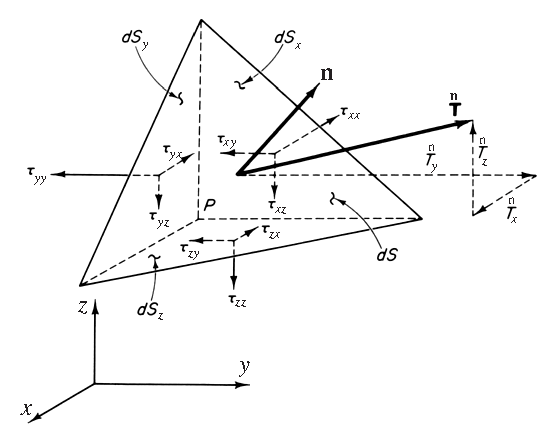
\includegraphics[width=0.5\textwidth]{Fung-3.7.eps}
\end{center}
\caption{Surface tractions on an elemental tetrahedron, vertex
  $P$. The unit outward normal of face $\cd S$ is $\bm{n}$, and on
  this face the traction vector is $\stackrel{\bm{n}}{\bm{T}}$.}
\label{fig.tetra}
\end{figure}

In the limit that the size of the tetrahedron goes to zero, then any
body forces associated with the volume of the tetrahedron (like
gravitational attraction) can be ignored relative to the surface
tractions, because the volume (proportional to length cubed) will
approach zero faster than areas (proportional to length squared). We
can also then assume that the stress tensor relevant to computing the
tractions is then uniform, because we are effectively using the value
at $P$. The equation of equilibrium of the tetrahedron in the $x$
direction is then
\[
-\tau_{xx}n_x\cd S -\tau_{yx}n_y\cd S -\tau_{zx}n_z\cd S +
 \stackrel{\bm{n}}{T}_x\cd S = 0,
\]
from which
\[
\stackrel{\bm{n}}{T}_x = \tau_{xx}n_x + \tau_{yx}n_y + \tau_{zx}n_z,
\]
while for the other two directions we will have 
\[
\stackrel{\bm{n}}{T}_y = \tau_{xy}n_x + \tau_{yy}n_y + \tau_{zy}n_z,\qquad
\stackrel{\bm{n}}{T}_z = \tau_{xz}n_x + \tau_{yz}n_y + \tau_{zz}n_z.
\]
We can write these relationships between tractions and the stress
tensor concisely in vector form as
\[
\stackrel{\bm{n}}{\bm{T}} = \bm{n\cdot\tau}.
\]

A very important point is that the stress tensor is symmetric, \ie
$\tau_{ij}=\tau_{ji}$, so that the matrix array of components written
above is symmetrical about the leading diagonal. This can be shown by
considering the moments of the tractions and body forces that apply to
a small volume of continuum. In figure~\ref{fig.para} we see stress
components acting on the faces of an infinitesimal parallelepiped of
material. Also, for generality, we allow for a body force $\bm{F}$ per
unit volume to act on the material. Taking equilibrium of moments of
the applied forces about the edge of the parallelepiped closest to the
$z$ axis, for example,
\begin{align*}
-&\left(\tau_{xx}+\frac{\partial\tau_{xx}}{\partial x}\Delta x\right)
 \Delta y\Delta z\frac{\Delta y}{2} +
 \tau_{xx}\Delta y\Delta z\frac{\Delta y}{2}\\
+&\left(\tau_{xy}+\frac{\partial\tau_{xy}}{\partial x}\Delta x\right)
 \Delta y\Delta z\Delta x -
 \left(\tau_{yx}+\frac{\partial\tau_{yx}}{\partial y}\Delta y\right)
 \Delta x\Delta z\Delta y\\
+&\left(\tau_{yy}+\frac{\partial\tau_{yy}}{\partial y}\Delta y\right)
 \Delta x\Delta z\frac{\Delta x}{2} -
 \tau_{yy}\Delta x\Delta z\frac{\Delta x}{2}\\
+&\left(\tau_{zy}+\frac{\partial\tau_{zy}}{\partial z}\Delta z\right)
 \Delta x\Delta y\frac{\Delta x}{2} -
 \tau_{zy}\Delta x\Delta y\frac{\Delta x}{2}\\
-&\left(\tau_{zx}+\frac{\partial\tau_{zx}}{\partial z}\Delta z\right)
 \Delta x\Delta y\frac{\Delta y}{2} +
 \tau_{zx}\Delta x\Delta y\frac{\Delta y}{2}\\
-&F_x\Delta x\Delta y\Delta z\frac{\Delta y}{2}
+F_y\Delta x\Delta y\Delta z\frac{\Delta x}{2} = 0.
\end{align*}
If we divide through by $\Delta V=\Delta x\Delta y\Delta z$, and take
limits as these lengths approach zero, we find that
$\tau_{xy}=\tau_{yx}$. Similar conclusions can be drawn for the other
two directions, showing that $\tau_{xz}=\tau_{zx}$ and
$\tau_{yz}=\tau_{zy}$.

\begin{figure}
\begin{center}
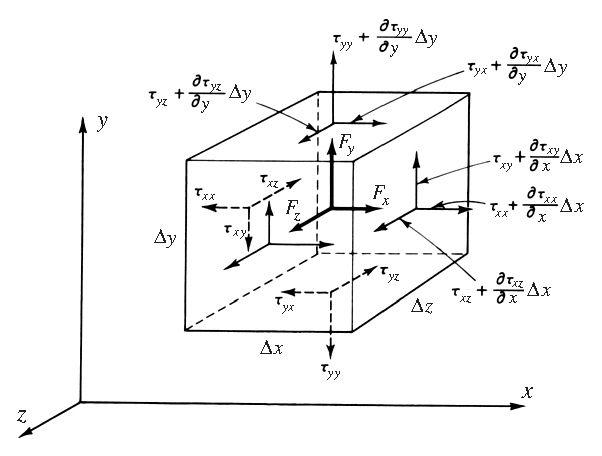
\includegraphics[width=0.5\textwidth]{Fung-3.8.eps}
\end{center}
\caption{Stress components on an infinitesimal parallelepiped. Body
  force components $F_x$, $F_y$, $F_z$ are also shown.}
\label{fig.para}
\end{figure}

So there are at most only 6 independent stress components of
$\bm{\tau}$ out of 9. The consequences of this symmetry are
far-reaching. For example, from matrix theory, we know that the
eigenvalues (or `principal stresses') of the stress tensor are all
real, and that the eigenvectors are mutually orthogonal. This means
that given the stress tensor components in some orthogonal coordinate
system, we will always be able to transform (through rotation) to a
new coordinate system also with orthogonal axes, in which the shear
stress components are zero, and the remaining normal stresses are the
principal stresses or the eigenvalues of the original stress
tensor. We will not pursue this point in more depth, but in general,
considerations of symmetry pervade continuum mechanics.

%=============================================================================
\subsection{Isotropic and deviatoric stress components}

%%%%%%%%%%%%%%%%%%%%%%%%%%%%%%%%%%%%%%%%%%%%%%%%%%%%%%%%%%%%%%%%%%%%%%%%%%%%%%
\section{Deformation of continua}

Now that we have the idea of a continuum, we can consider describing
its motion. Instead of the motion of single points or of rigid bodies,
we use the idea of a `field' description of displacements, velocities
and accelerations, where the values can vary continuously from point
to point in space.

%=============================================================================
\subsection{The deformation field and the infinitesimal strain and
  rotation tensors}

The idea of a strain expresses how lengths within a material change
when the material is deformed. Consider the position of a point in a
continuum specified by $\bm{x}=(x, y, z)$. If the continuum is
deformed by a small amount $\bm{u}(\bm{x})=(u, v, w)(x, y, z)$, \ie by
a deformation field that may vary with position, then the new location
of the point after deformation is
$\bm{x}^\prime=\bm{x}+\bm{u}(\bm{x})$. Now we also consider the
deformation of a point that is close to $\bm{x}$, \ie
$\bm{x}+\cd\bm{x}$. After the motion it will be in a new position
\[
\bm{x}^\prime + \cd\bm{x}^\prime + \bm{u}(\bm{x}+\cd\bm{x}).
\]

Since we are considering only an infinitesimally small motion, we can
approximate this by using the first two terms in the Taylor series
expansion, which we will write for all three components of deformation
\begin{align*}
x^\prime + \cd x^\prime & \approx x +\cd x +
 \frac{\partial u}{\partial x}\,\cd x +
 \frac{\partial u}{\partial y}\,\cd y +
 \frac{\partial u}{\partial z}\,\cd z,\\
y^\prime + \cd y^\prime & \approx y +\cd y +
 \frac{\partial v}{\partial x}\,\cd x +
 \frac{\partial v}{\partial y}\,\cd y +
 \frac{\partial v}{\partial z}\,\cd z,\\
z^\prime + \cd z^\prime & \approx z +\cd z +
 \frac{\partial w}{\partial x}\,\cd x +
 \frac{\partial w}{\partial y}\,\cd y +
 \frac{\partial w}{\partial z}\,\cd z.
\end{align*}
The concise vector form of this is
\[
\bm{x}^\prime + \cd\bm{x}^\prime=
\bm{x}+(\bm{I}+\bm{\nabla u})\bm{\cdot}\cd{\bm{x}},
\]
where $\bm{I}$ is the $3\times3$ identity matrix, and is not
associated with deformation: $\bm{I}\,\cd\bm{x}$ represents the
original infinitesimal length. Note the equivalence between the
coordinate-free expression $\bm{\nabla u}$ and the $3\times3$ array of
partial derivatives above. We will stay with this form temporarily. To
make further progress we decompose this (tensor) operator $\bm{\nabla
u}$ into symmetric and anti-symmetric parts: from the standard means
of doing this for a matrix $A=(A+A^T)/2+(A-A^T)/2$, where $^T$ is the
transpose operation (reflection about the leading diagonal) we can
write
\[
\bm{\nabla u} =
 \frac{1}{2}\left[\bm{\nabla u}+(\bm{\nabla u})^T\right]+
 \frac{1}{2}\left[\bm{\nabla u}-(\bm{\nabla u})^T\right].
\]
The first term on the right-hand-side is the symmetric part of
$\bm{\nabla u}$ while the second is the anti-symmetric part. Expanding
back out again we have 
\begin{multline}
\begin{bmatrix}
 \frac{\partial u}{\partial x}&
 \frac{\partial u}{\partial y}&
 \frac{\partial u}{\partial z}\\
 \frac{\partial v}{\partial x}&
 \frac{\partial v}{\partial y}&
 \frac{\partial v}{\partial z}\\
 \frac{\partial w}{\partial x}&
 \frac{\partial w}{\partial y}&
 \frac{\partial w}{\partial z}\\
\end{bmatrix}
\begin{pmatrix}
\cd x \\ \cd y \\ \cd z
\end{pmatrix}
=\\
\begin{bmatrix}
 \frac{\partial u}{\partial x}&
 \frac{1}{2}(\frac{\partial u}{\partial y}+\frac{\partial v}{\partial x})&
 \frac{1}{2}(\frac{\partial u}{\partial z}+\frac{\partial w}{\partial x})\\
 \frac{1}{2}(\frac{\partial v}{\partial x}+\frac{\partial u}{\partial y})&
 \frac{\partial v}{\partial y}&
 \frac{1}{2}(\frac{\partial v}{\partial z}+\frac{\partial w}{\partial y})\\
 \frac{1}{2}(\frac{\partial w}{\partial x}+\frac{\partial u}{\partial z})&
 \frac{1}{2}(\frac{\partial w}{\partial y}+\frac{\partial v}{\partial z})&
 \frac{\partial w}{\partial z}\\
\end{bmatrix}
\begin{pmatrix}
\cd x \\ \cd y \\ \cd z
\end{pmatrix}
+\\
\begin{bmatrix}
 0 &
 \frac{1}{2}(\frac{\partial u}{\partial y}-\frac{\partial v}{\partial x})&
 \frac{1}{2}(\frac{\partial u}{\partial z}-\frac{\partial w}{\partial x})\\
 \frac{1}{2}(\frac{\partial v}{\partial x}-\frac{\partial u}{\partial y})&
 0 &
 \frac{1}{2}(\frac{\partial v}{\partial z}-\frac{\partial w}{\partial y})\\
 \frac{1}{2}(\frac{\partial w}{\partial x}-\frac{\partial u}{\partial z})&
 \frac{1}{2}(\frac{\partial w}{\partial y}-\frac{\partial v}{\partial z})&
 0\\
\end{bmatrix}
\begin{pmatrix}
\cd x \\ \cd y \\ \cd z
\end{pmatrix}.
\label{eq.decomp}
\end{multline}
(And we can see why more compact notations are preferred!) Note the
respective symmetry and anti-symmetry of the two matrices on the
right-hand-side of this expression. Now if first we examine in detail
the final term in this equation, we find that the components in it are
exactly equivalent to those of the vector cross product
$\frac{1}{2}\bm{\omega}\times\cd \bm{x}$, where $\omega_{x}=\partial
w/\partial y - \partial v/\partial z$, etc.\ (or in full
$\bm{\omega}=\bm{\nabla}\times\bm{u}$). In turn this means that the
displacement it causes is exactly equivalent to an infinitesimal
solid-body rotation through angle $\frac{1}{2}\bm{\omega}$. But a
solid-body rotation by definition causes no distortion of the body
concerned. Therefore only the first term in the right-hand-side of
equation (\ref{eq.decomp}), due to the symmetric part of $\bm{\nabla
u}$, produces distortion (and, as we will see later, is associated
with stress in solids). This symmetric part (with at most 6
independent terms out of 9) is called the infinitesimal strain
tensor. The other, anti-symmetric part (with at most 3 independent
terms out of 9), is called the infinitesimal rotation tensor.

The notation we will use for the infinitesimal strain tensor is
$\bm{e}\equiv e_{ij}=(\partial u_i/\partial x_j + \partial
u_j/\partial x_i)/2$ with indices $i$ and $j$ taken to mean any of
$x$, $y$ or $z$ (equivalently 1, 2 or 3). It should be noted that this
refers to an \emph{infinitesimal} strain. The expressions for finite
strains are more complicated, and non-linear, but we can do quite a
lot of useful analysis based on $\bm{e}$, simply because the relative
amount of deformation prior to failure is often quite small in solid
materials. We note also that since $\bm{e}$ is a real, symmetric
tensor, it has exactly the same mathematical properties as the stress
tensor: it is guaranteed to have real eigenvalues (the `principal
strains'), and we can always find a system of three mutually
orthogonal planes on which the shear strains (the off-diagonal terms)
are zero.

%=============================================================================
\subsection{The velocity field}

In fluid mechanics, it is the velocity field, rather than the
displacement field, that is of central interest. In large part this is
because the strains, \ie gradients of displacement, rapidly become
large and non-linearly dependent on displacement, so that analysis
based on displacements quickly becomes impossible in any practicable
sense. If instead, we focus on velocity, we find that the gradients of
velocity, itself an infinitesimal measure, always depend linearly on
velocity, no matter how large this is.  (Of course, we do not get
something for nothing, and as we shall see, it turns out that instead
the equations of motion themselves can become non-linearly dependent
on velocity.) Another central reason for focusing on velocity stems
from the fact that fluids in equilibrium cannot resist a shear stress,
whereas in steady motion, they can.

Consider the relative velocity $\cd\bm{u}$ between two neighbouring
points fixed in space at $\bm{x}$ and $\bm{x}+\cd\bm{x}$. Then, using
the chain rule, the difference in velocities at the two points is
$\cd\bm{u}=\bm{\nabla u\cdot}\cd\bm{x}$, which has exactly the same
form as the left-hand-side of equation (\ref{eq.decomp}). As before,
we split the gradient tensor $\bm{\nabla u}$ into symmetric and
anti-symmetric parts, and come up with an expression that has exactly
the same form as the right-hand-side of (\ref{eq.decomp}). Analogous
to the symmetric strain tensor $\bm{e}$, we have the symmetric
\emph{rate of strain} tensor $\bm{S}$, while the anti-symmetric part
$\bm{\Omega}$ is often called the rate of rotation or \emph{spin}
tensor, as it is related directly to the vorticity vector
$\bm{\nabla}\times\bm{u}$ that expresses the local rotation rate. Note
that it is common to use the same symbol, $\bm{u}$, to express either
the displacement field in solid mechanics, or the velocity field in
fluid mechanics. In practice, it is usually clear which is meant,
since we typically deal either with one or the other in a specific
problem. Of course, when the problem involves coupled fluid flow and
distortion of solid material, we need to distinguish the two with
different symbols.

Now the rate of strain $\bm{S}$, which is again a real symmetric
tensor, shares the mathematical properties of the stress tensor
$\bm{\tau}$ and the infinitesimal strain tensor $\bm{e}$; it has three
real eigenvalues (or principal rates of strain), and we can always
find three mutually orthogonal planes on which the shear rates of
strain are zero.

%=============================================================================
\subsection{Lagrangian and Eulerian descriptions of time rates of
  change}

When dealing with time rates of change in continua, it is important to
distinguish between the local time rate of change, and the time rate
of change `following the motion', or associated with a specific piece
of material as it moves. In the dynamics of points and rigid bodies,
we are used to talking about the second of these two concepts as if it
were \emph{the} time rate of change, but we need to be more careful
now because we are dealing with partial derivatives.

Firstly, if we are interested in the rate of change of something, say
the scalar concentration $c$ at a fixed point in space, then the
partial derivative $\partial c/\partial t$, where $t$ is time, is the
`local' time rate of change of $c$, \ie what is seen by an observer
locally fixed in space. \citet*{bsl62} give the example of the
concentration of fish in a river as seen by an observer sitting on a
bridge, and looking down at one point in the river.

Next, supposing we get in a motorboat and speed around on the river,
and observe the concentration of fish from the boat. Then the time
rate of change of $c$ is the `total time derivative', which, using the
chain rule, is
\begin{equation}
\frac{\cd c}{\cd t} = \frac{\partial c}{\partial t}+
\frac{\partial c}{\partial x}\frac{\cd x}{\cd t}+
\frac{\partial c}{\partial y}\frac{\cd y}{\cd t}+
\frac{\partial c}{\partial z}\frac{\cd z}{\cd t},
\label{eq.total}
\end{equation}
where the spatial partial derivatives $\partial c/\partial x$, etc.\
describe how the concentration varies in space at a fixed time, and
$\cd x/\cd t$ etc.\ describe the velocity of the boat.

Finally, consider the case where we let the boat drift downstream so
that it moves (`convects') with the local fluid velocity $\bm{u} = (u,
v, w)$. Then we have a special case of (\ref{eq.total}) and to reflect
this specialisation we use a new differentiation symbol
\begin{equation}
\frac{\cD c}{\cD t} = \frac{\partial c}{\partial t}+
u\frac{\partial c}{\partial x}+
v\frac{\partial c}{\partial y}+
w\frac{\partial c}{\partial z}\equiv
\frac{\partial c}{\partial t}+\bm{u\cdot\nabla}c
\label{eq.material}
\end{equation}
This specialised total time derivative $\cD/\cD t$ is variously called
the `substantial derivative', `material derivative' (both stemming
from the idea that we associate it with a particular piece of
material/substance as we drift with the flow), or `derivative
following the motion'. Note that now, in addition to the local time
rate of change $\partial c/\partial t$, there is a new rate of change
$\bm{u\cdot\nabla}c$ which is called the `convective', or sometimes,
`advective', rate of change. Even when $\partial c/\partial t=0$, \ie
the concentration is steady everywhere in time, if we follow the
motion of the material of the continuum, we can still see a time rate
of change of fish concentration depending on how this varies in space
at a fixed time.

The two different approaches to describing the time rate of change
expressed in (\ref{eq.material}) are known as the `Lagrangian'
description $\cD(\,)/\cD t$, where we follow the motion of a tagged
piece of material, and the `Eulerian' description,
$\partial(\,)/\partial t+\bm{u\cdot\nabla}(\,)$, where the derivatives
are based on measures taken in a fixed frame of reference. Partly
because it fits more naturally with both experimental and typical
mesh-based computational methods, the Eulerian description is more
commonly used in continuum mechanics. The Lagrangian description is
more commonly used when dealing with the mechanics of rigid bodies.

%=============================================================================
\subsection{The acceleration of a particle}

The concepts of local, convective, and material rates of change also
apply when we need to work with the acceleration of material, except
that the acceleration is of course a vector quantity. Taking the
material derivative of the velocity because we are interested in the
acceleration of a particle of material
\[
\bm{a}=\frac{\cD\bm{u}}{\cD t}=
  \frac{\partial\bm{u}}{\partial t}+
  \left(u\frac{\partial\bm{u}}{\partial x}+
        v\frac{\partial\bm{u}}{\partial y}+
        w\frac{\partial\bm{u}}{\partial z}\right)=
  \frac{\partial\bm{u}}{\partial t}+\bm{u\cdot\nabla u}
,
\]
where again we see the split between the local and convective
acceleration.  Because of its importance, we will expand this vector
expression out in Cartesian components:
\begin{alignat*}{7}
a_x&=\frac{\partial u}{\partial t}&+&
    u\frac{\partial u}{\partial x}&+&
    v\frac{\partial u}{\partial y}&+&
    w\frac{\partial u}{\partial z},\\
a_y&=\frac{\partial v}{\partial t}&+&
    u\frac{\partial v}{\partial x}&+&
    v\frac{\partial v}{\partial y}&+&
    w\frac{\partial u}{\partial z},\\
a_z&=\frac{\partial w}{\partial t}&+&
    u\frac{\partial w}{\partial x}&+&
    v\frac{\partial w}{\partial y}&+&
    w\frac{\partial w}{\partial z}.
\end{alignat*}
Note that the convective part of this Eulerian description of the
acceleration field depends non-linearly on the velocity.

%%%%%%%%%%%%%%%%%%%%%%%%%%%%%%%%%%%%%%%%%%%%%%%%%%%%%%%%%%%%%%%%%%%%%%%%%%%%%%
\section{Transport phenomena}

As well as forces (stresses) and deformation, another central focus in
continum mechanics is the transport of conserved quantities such as
mass, momentum, energy. The two main means of transport are advection,
\ie direct transport by being carried with a flow, and molecular
diffusion brought about by random motion of molecules.

%=============================================================================
\subsection{The volume and mass rate of flow}

The volume rate of flow $Q$ through an (imaginary) surface in a flow
field is a fundamentally important quantity. Now the direction of the
flow relative to the direction of the surface must be
considered. Refer to figure~\ref{fig.flowQ}. Naturally, if the flow
direction is parallel to the surface (\ie if the velocity $\bm{u}$ is
itself normal parallel to the unit outward normal $\bm{n}$), then
there is \emph{no} volume flow through the surface, while if the flow
direction matches that of the unit outward normal $\bm{n}$ to the
surface, then the volume flow through the surface is
maximised. Evidently the volume flow rate (volume swept through per
unit time) $\cd Q$ through a small element of surface $\cd A$ depends
on the cosine of the angle $\theta$ between the velocity vector and
the unit outward normal, which we can simply express through a vector
dot product:
\[
\cd Q=|\bm{u}| \cos(\bm{n}, \bm{u})\,\cd A = \bm{u\cdot n}\,\cd A,
\]
while the total volume flow rate $Q$ through surface $S$ is then
\[
Q = \int_S \bm{u\cdot n}\,\cd A.
\]

\begin{figure}
\begin{center}
%\begin{tabular}{cccc}
%\raisebox{8ex}{(\textit{a})} &
%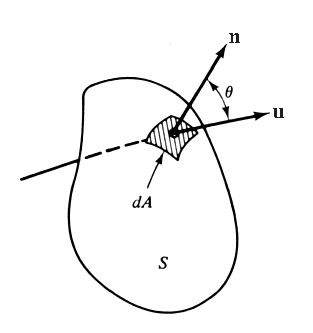
\includegraphics[width=0.25\textwidth]{White-1.3a.eps} &
%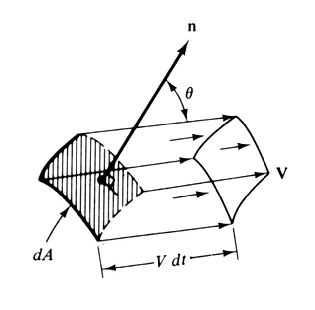
\includegraphics[width=0.25\textwidth]{White-1.3b.eps} &
%\raisebox{8ex}{(\textit{b})}
%\end{tabular}
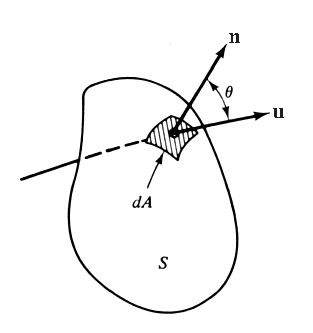
\includegraphics[width=0.25\textwidth]{White-1.3a.eps}
\end{center}
\caption{The rate of flow swept through a surface. \citep[From][]{white86}}
\label{fig.flowQ}
\end{figure}

Since the amount of mass in an elemental volume is the density times
the volume, the rate of mass flow across $S$ is
\[
\dot{m}=\int_S \rho\bm{u\cdot n}\,\cd A.
\]


%%%%%%%%%%%%%%%%%%%%%%%%%%%%%%%%%%%%%%%%%%%%%%%%%%%%%%%%%%%%%%%%%%%%%%%%%%%%%%
\section{Diffusion and diffusive flux}

Diffusion occurs through random motion of molecules, and is driven by
a tendency to statistical uniformity, \ie a state of statistical
equilibrium. In order for diffusive transport to occur, all that is
needed is a spatial gradient of concentration of some property. Unlike
transport associated directly with the velocity field, diffusive
transport will occur in a direction normal to a surface even if there
is no component of the bulk velocity normal to the surface, so long as
there is a concentration gradient across it.

The `property' with which diffusive flux is associated depends on the
conserved quantity under investigation. It may be the total amount of
a scalar (\eg solute, reactant); it may be heat; it may be momentum.
In order to make a differential formulation we deal with the
concentration of the conserved quantity, either per unit volume or per
unit mass.

Suppose we take the property of interest be the total amount of a
scalar, with concentration $c$ per unit volume. Then the simplest
assumption for the flux $\bm{f}$ of the scalar owing to diffusion is
that it is related the the gradient $\nabla c$ through a simple linear
relationship with a single \emph{transport coefficient} $k$
\[
\bm{f}=-k\nabla c = -k \left(
 \frac{\partial c}{\partial x},
 \frac{\partial c}{\partial y},
 \frac{\partial c}{\partial z}
\right),
\]
where we have written the Cartesian components of $\nabla c$ in the
final parenthesised expression. The negative sign expresses the idea
that the direction of diffusive flux is from a region of high
concentration to a region of low concentration. If we wish to know how
fast the total amount of the quantity associated with $c$ is
transported across a small area $\cd A$, then the situtation is much
the same as shown in figure~\ref{fig.flowQ}, except that the diffusive
flux $\bm{f}$ replaces the velocity. Thus the diffusive flux through
$\cd A$ of the quantity concerned is
\[
\bm{f\cdot n}\,\cd A.
\]

If the quantity concerned is momentum, then the concentration of
momentum per unit volume is $\rho\bm{u}$ (note: a vector) and for
diffussion of momentum the transport coefficient is the viscosity of the
fluid, $\mu$.


















%#############################################################################
\chapter{Conservation Laws in continuum form}
\label{ch.cons}

Conservation laws are really fundamental hypotheses based on our
experience. They cannot be independently proven; \citet{feynman67}
gives an excellent discussion of our understanding of physical
laws. We will examine conservation of mass, a passive scalar, and
momentum. Another conservation law can be written for conservation of
energy, but we will not examine this in continuum form. 
%We will generally regard the materials as being of constant density.

The conservation laws will be derived in a Cartesian coordinate
system, but where appropriate we will give the equivalent
coordinate-free (or vector-notation) result. The method of
presentation follows that of \citet*{bsl62}; for much more complete
accounts see \citet{aris62,bat67,fung69}.

%%%%%%%%%%%%%%%%%%%%%%%%%%%%%%%%%%%%%%%%%%%%%%%%%%%%%%%%%%%%%%%%%%%%%%%%%%%%%%
\section{Conservation of mass}

Consider the mass balance for a stationary volume element $\Delta
V=\Delta x\Delta y\Delta z$ through which fluid is flowing, as shown
in figure~\ref{fig.massV}. For the present we will allow the density
$\rho$ to vary in time and space. The law of mass conservation is that
mass is neither created nor destroyed, but is conserved. For the
volume element, we write this in words as
\begin{equation}
\left\{ \parbox{23mm}{rate of mass\\ accumulation} \right\}=
\left\{ \parbox{23mm}{rate at which\\ mass flows in} \right\}-
\left\{ \parbox{25mm}{rate at which\\ mass flows out} \right\}.
\label{eq.mass_bal_words}
\end{equation}
When the system is in steady state, the left-hand-side of this
equation must be zero.  First considering the flow rates through the
faces normal to the $x$-direction, the rate at which mass flows in is
$(\rho u)|_x \Delta y\Delta z$, while the rate at which it flows out
is $(\rho u)|_{x + \Delta x} \Delta y\Delta z$. We can write similar
expressions for the $y$ and $z$ directions (where the the velocity
components are respectively $v$ and $w$), while the rate of
accumulation of mass inside the element is $(\partial \rho/\partial
t)\Delta x\Delta y\Delta z$. (The notation $()|_x$ means `evaluated at
location $x$'.)

\begin{figure}
\begin{center}
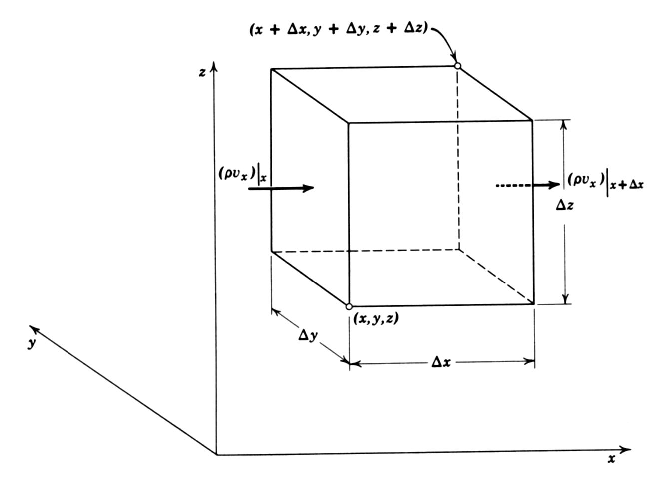
\includegraphics[width=0.5\textwidth]{BSL-3.1-1.eps}
\end{center}
\caption{A  finite elemental volume $\Delta V=\Delta x\Delta y\Delta z$
with flow through its faces.}
\label{fig.massV}
\end{figure}

The mathematical expression of the mass balance
equation~(\ref{eq.mass_bal_words}) is then 
\begin{equation}
\begin{split}
\Delta x\Delta y\Delta z\frac{\partial \rho}{\partial t}=&
  \Delta y\Delta z[(\rho u)|_{x}-(\rho u)|_{x+\Delta x}]+\\
& \Delta x\Delta z[(\rho v)|_{y}-(\rho v)|_{y+\Delta y}]+\\
& \Delta x\Delta y[(\rho w)|_{z}-(\rho w)|_{z+\Delta z}].
\end{split}
\end{equation}
Dividing through by $\Delta V=\Delta x\Delta y\Delta z$ and taking
limits as the lengths go to zero, we get
\begin{equation}
\frac{\partial \rho}{\partial t}=-\left(
\frac{\partial \rho u}{\partial x} +
\frac{\partial \rho v}{\partial y} +
\frac{\partial \rho w}{\partial z}\right).
\end{equation}
Using the chain rule we can rearrange this as
\begin{equation}
\frac{\partial \rho}{\partial t} + u\frac{\partial\rho}{\partial x} +
v\frac{\partial\rho}{\partial y}+w\frac{\partial\rho}{\partial z}=-\rho\left(
\frac{\partial u}{\partial x} +
\frac{\partial v}{\partial y} +
\frac{\partial w}{\partial z}\right),
\label{eq.contin}
\end{equation}
which from the definition of the material derivative we recognise as 
\begin{equation}
\frac{\cD \rho}{\cD t} =-\rho\left(
\frac{\partial u}{\partial x} +
\frac{\partial v}{\partial y} +
\frac{\partial w}{\partial z}\right),
\end{equation}
or, in vector notation,
\begin{equation}
\frac{\cD \rho}{\cD t} =-\rho\bm{\nabla\cdot u}.
\end{equation}
This tells us that the rate of change of density following a particle
of fluid is the negative of the divergence or dilatation of the
velocity field. For the applications we will discuss, we can take
$\cD\rho/\cD t=0$, and use the fact that then $\bm{\nabla\cdot
u}=0$\,---\,flows with this property are called
incompressible. Simplifying even further we could take
$\rho=\textrm{constant}$, which is philosophically slightly different,
but has the same consequence for the divergence of velocity.

%%%%%%%%%%%%%%%%%%%%%%%%%%%%%%%%%%%%%%%%%%%%%%%%%%%%%%%%%%%%%%%%%%%%%%%%%%%%%%
\section{Conservation of a scalar}

Now supposing we wish to examine the fluid transport of a passive
scalar (\ie one that is not created or destroyed, say by chemical
reaction, within the continuum). If we are concerned with the
transport of heat, temperature would be the appropriate scalar, but in
biomedical applications it is usually the concentration of a
solute. The concentration of the scalar per unit volume is denoted by
$c$. Now we have to allow for diffusion of the scalar down its
concentration gradient by molecular-level interactions, as well as
convective transport by the fluid velocity field. As defined
previously, the diffusive flux is $\bm{f}=-k\nabla c$, where $k$ is
the diffusivity of $c$.

In words, the law of conservation of a passive
scalar for a fixed control volume is
\begin{equation}
\left\{ \parbox{23mm}{rate of\\ scalar\\ accumulation} \right\}=
\left\{ \parbox{15mm}{rate at\\ which scalar flows in} \right\}-
\left\{ \parbox{15mm}{rate at\\ which scalar flows out} \right\}+
\left\{ \parbox{17mm}{rate at\\ which scalar diffuses in} \right\}-
\left\{ \parbox{20mm}{rate at\\ which scalar diffuses out} \right\}.
\label{eq.scalar_bal_words}
\end{equation}
Again with reference to the elemental fixed geometry of
figure~\ref{fig.massV}, we can write this as
\begin{multline}
\Delta x\Delta y\Delta z\frac{\partial c}{\partial t}=
\Delta y\Delta z\left[(c u)|_{x}-(c u)|_{x+\Delta x}\right]+
\Delta x\Delta z\left[(c v)|_{y}-(c v)|_{y+\Delta y}\right]+\\
\Delta x\Delta y\left[(c w)|_{z}-(c w)|_{z+\Delta z}\right]+\\
\Delta y\Delta z\left[(k \frac{\partial c}{\partial x})|_{x}-(k
  \frac{\partial c}{\partial x})|_{x+\Delta x}\right]+
\Delta x\Delta z\left[(k \frac{\partial c}{\partial y})|_{y}-(k
  \frac{\partial c}{\partial y})|_{y+\Delta y}\right]+\\
\Delta x\Delta y\left[(k \frac{\partial c}{\partial z})|_{z}-(k
  \frac{\partial c}{\partial z})|_{z+\Delta y}\right].
\end{multline}
Dividing by $\Delta V$ and taking limits, we have
\begin{equation}
\frac{\partial c}{\partial t}=
-\left(\frac{\partial cu}{\partial x}+\frac{\partial cv}{\partial
  y}+\frac{\partial cw}{\partial z}\right) + \frac{\partial}{\partial
  x}\left(k\frac{\partial c}{\partial x}\right)+ \frac{\partial}{\partial
  y}\left(k\frac{\partial c}{\partial y}\right)+ \frac{\partial}{\partial
  z}\left(k\frac{\partial c}{\partial z}\right),
\end{equation}
or, using the chain rule and rearranging,
\begin{equation}
\frac{\cD c}{\cD t}=
-c\left(\frac{\partial u}{\partial x}+\frac{\partial v}{\partial
  y}+\frac{\partial w}{\partial z}\right) + \frac{\partial}{\partial
  x}\left(k\frac{\partial c}{\partial x}\right)+ \frac{\partial}{\partial
  y}\left(k\frac{\partial c}{\partial y}\right)+ \frac{\partial}{\partial
  z}\left(k\frac{\partial c}{\partial z}\right).
\end{equation}
Such an equation is commonly called an `advection--diffusion' equation
for the concentration, or more simply a transport equation for the
scalar.  Now if also we assume $k=\textrm{constant}$ and
$\bm{\nabla\cdot u}=0$ (incompressible flow) we have
\begin{equation}
\frac{\cD c}{\cD t}=
k\left(\frac{\partial^2 c}{\partial x^2} + \frac{\partial^2
  c}{\partial y^2}+ \frac{\partial^2 c}{\partial z^2}\right)=
k\nabla^2 c.
\end{equation}
If the scalar is not passive, but may be created or destroyed within
the control volume by a reaction, this could be dealt with by adding a
creation rate $\dot{c}$ to the right-hand-side of this equation:
\begin{equation}
\frac{\cD c}{\cD t}=
k\nabla^2 c + \dot{c}(\bm{x}).
\end{equation}
Naturally, if the creation is reaction-dependent, this rate might in
reality be dependent on the local concentrations of a set of other
scalars, in which case we would have a coupled set of scalar transport
equations.

%%%%%%%%%%%%%%%%%%%%%%%%%%%%%%%%%%%%%%%%%%%%%%%%%%%%%%%%%%%%%%%%%%%%%%%%%%%%%%
\section{Conservation of momentum}

The equation for conservation of momentum is nothing more than
Newton's Second Law written for a continuum. We have to allow for
two kinds of forces: `body forces' which act in a distributed sense
(\eg due to graviational attraction), and `surface forces' or
tractions, which act on surfaces of a volume as a result of internal
stress.  Like velocity and acceleration, momentum is a vector
property, so we will end up with a set of three scalar equations, one
for each component of momentum.

Note: as was pointed out in the previous chapter, a traction is not
the same as a stress: a traction is a vector, or a first-order tensor,
whereas a stress is a second-order tensor. Often the two things are
discussed without making the distinction, but to derive a traction
from a stress we need to know both the stress field and the
orientation of the surface on which the traction acts. The tractions
are produced by molecular-level effects\,---\,in a fluid, by molecular
diffusion of momentum, and in a solid by inter-molecular forces.

%It is
%conventional and convenient to decompose the state of stress into an
%`isotropic' component, that is the same in all directions, and a
%non-isotropic or `deviatoric' component that encapsulates the tensor
%behaviour. From everyday experience we are used to the isotropic
%component: it is the pressure, and stems fundamentally from
%compression of the material. In fluids, the deviatoric component of
%the stress is produced by shear and viscosity.

In words, the expression for conservation of momentum for a volume
fixed in space is
\begin{equation}
\left\{ \parbox{23mm}{rate of\\ momentum\\ accumulation} \right\}=
\left\{ \parbox{19mm}{rate of\\ momentum\\ in} \right\}-
\left\{ \parbox{19mm}{rate of\\ momentum\\ out} \right\}+
\left\{ \parbox{25mm}{sum of forces acting on\\ system} \right\}.
\label{eq.mom_bal_words}
\end{equation}
For a steady-state system, the left-hand-side of this equation is
zero.

\begin{figure}
\begin{center}
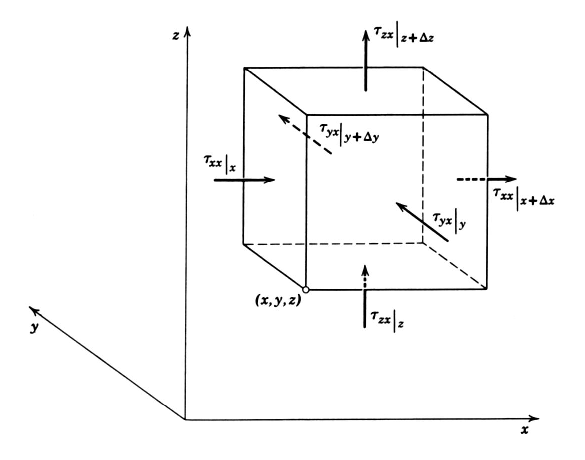
\includegraphics[width=0.5\textwidth]{BSL-3.1-2.eps}
\end{center}
\caption{A finite elemental volume $\Delta V=\Delta x\Delta y\Delta z$
with surface tractions acting on its faces.}
\label{fig.momV}
\end{figure}

We will start with $x$-component momentum per unit mass (locally,
$\rho u$).  Consider the elemental volume $\Delta V=\Delta x\Delta
y\Delta z$ shown in figure~\ref{fig.momV}. The rate at which
$x$-component momentum accumulates within $\Delta V$ is $\Delta
V\partial \rho u/\partial x$. The rate at which $x$-component momentum
convects into the face at $x$ is given by $\rho uu|_{x}\Delta y\Delta
z$; the rate at which it convects out at $x+\Delta x$ is $\rho
uu|_{x+\Delta x}\Delta y\Delta z$. The rate at which it enters at $y$
is $\rho uv|_y$; note the $y$-component velocity, $v$, carries
$x$-component momentum here. Adding up the convective contributions to
$x$-momentum of all six faces
\begin{equation}
\Delta y\Delta z(\rho uu|_x-\rho uu|_{x+\Delta x})+\Delta x\Delta
z(\rho uv|_y-\rho uv|_{y+\Delta y})+\Delta x\Delta y(\rho uw|_z-\rho
uw|_{z+\Delta z}).
\end{equation}
Next we consider the $x$-component tractions acting on the six
faces. The deviatoric tractions have two indices, \eg $\tau_{yx}$ is
the traction on a face normal to the $y$ direction and which points in
the $x$ direction. Note that $\tau_{xx}$ is a traction acting normal
to a face of our elemental volume, while $\tau_{yx}$ and $\tau_{zx}$
act tangentially to the faces on which they apply. Adding up the
%isotropic and deviatoric 
$x$-direction contributions on the six faces, we get
\begin{equation}
\Delta y\Delta z([\tau_{xx}]|_x-[\tau_{xx}]|_{x+\Delta x})+\Delta x\Delta
z(\tau_{yx}|_y-\tau_{yx}|_{y+\Delta y})+\Delta x\Delta
y(\tau_{zx}|_z-\tau_{zx}|_{z+\Delta z}).
\end{equation}
The typical distributed or body force is that due to gravity, which,
if there is a component $g_x$ in the $x$-direction, we can write as
$\rho g_x \Delta x\Delta y\Delta z$.

If we now assemble all the terms in the $x$-component equation for
conservation of momentum in the finite fixed control volume $\Delta V$
(\ref{eq.mom_bal_words}), divide through by $\Delta x\Delta y\Delta z$
and take the limit as these lengths approach zero, we get
\begin{equation}
\frac{\partial}{\partial t}\rho u=
-\left(
\frac{\partial}{\partial x}\rho uu+
\frac{\partial}{\partial y}\rho uv+
\frac{\partial}{\partial z}\rho uw
\right)
-\left(
\frac{\partial}{\partial x}\tau_{xx}+
\frac{\partial}{\partial y}\tau_{yx}+
\frac{\partial}{\partial z}\tau_{zx}
\right)
%-\frac{\partial p}{\partial x}
+\rho g_x.
\end{equation}
Similarly, the equations for the $y$- and $z$-components of momentum are
\begin{equation}
\frac{\partial}{\partial t}\rho v=
-\left(
\frac{\partial}{\partial x}\rho vu+
\frac{\partial}{\partial y}\rho vv+
\frac{\partial}{\partial z}\rho vw
\right)
-\left(
\frac{\partial}{\partial x}\tau_{xy}+
\frac{\partial}{\partial y}\tau_{yy}+
\frac{\partial}{\partial z}\tau_{zy}
\right)
%-\frac{\partial p}{\partial y}
+\rho g_y,
\end{equation}
\begin{equation}
\frac{\partial}{\partial t}\rho w=
-\left(
\frac{\partial}{\partial x}\rho wu+
\frac{\partial}{\partial y}\rho wv+
\frac{\partial}{\partial z}\rho ww
\right)
-\left(
\frac{\partial}{\partial x}\tau_{xz}+
\frac{\partial}{\partial y}\tau_{yz}+
\frac{\partial}{\partial z}\tau_{zz}
\right)
%-\frac{\partial p}{\partial z}
+\rho g_z.
\end{equation}

We can now use the chain rule on terms like $\partial \rho u/\partial
t$ and $\partial \rho u u/\partial x$, perform some rearrangement, and
use the continuity equation (\ref{eq.contin}) in order to arrive at
\begin{align}
\rho\frac{\cD u}{\cD t}=\rho\frac{\partial u}{\partial t} + 
\rho u\frac{\partial u}{\partial x} +
\rho v\frac{\partial u}{\partial y} +
\rho w\frac{\partial u}{\partial z} =&
%-\frac{\partial p}{\partial x} -
\left(
\frac{\partial \tau_{xx}}{\partial x} +
\frac{\partial \tau_{yx}}{\partial y} +
\frac{\partial \tau_{zx}}{\partial z}
\right)
\rho g_x,\\
\rho\frac{\cD v}{\cD t}=\rho\frac{\partial v}{\partial t} + 
\rho u\frac{\partial v}{\partial x} +
\rho v\frac{\partial v}{\partial y} +
\rho w\frac{\partial v}{\partial z} =&
%-\frac{\partial p}{\partial y} -
\left(
\frac{\partial \tau_{xy}}{\partial x} +
\frac{\partial \tau_{yy}}{\partial y} +
\frac{\partial \tau_{zy}}{\partial z}
\right)
+\rho g_y,\\
\rho\frac{\cD w}{\cD t}=\rho\frac{\partial w}{\partial t} + 
\rho u\frac{\partial w}{\partial x} +
\rho v\frac{\partial w}{\partial y} +
\rho w\frac{\partial w}{\partial z} =&
%-\frac{\partial p}{\partial z} -
\left(
\frac{\partial \tau_{xz}}{\partial x} +
\frac{\partial \tau_{yz}}{\partial y} +
\frac{\partial \tau_{zz}}{\partial z}
\right)
+\rho g_z.
\end{align}
Using vector notation we can write this set in coordinate-free form as
\begin{equation}
\rho\frac{\cD\bm{u}}{\cD t}=%-\nabla p
\bm{\nabla\cdot\tau} + \rho\bm{\cg}.
\label{eq.momvec}
\end{equation}
In words, this reads
\begin{equation}
\left\{ \parbox{23mm}{mass per unit volume times acceleration} \right\}=
%\left\{ \parbox{23mm}{pressure force per\\ unit volume} \right\}+
\left\{ \parbox{25mm}{%deviatoric 
                      stress force \\
                      per\\ unit volume} \right\} +
\left\{ \parbox{25mm}{gravitational force per unit volume} \right\}.
\label{eq.newt2_words}
\end{equation}
which is a statement of Newton's Second Law in the form
`mass$\times$acceleration = sum of forces', but expressed in continuum
form.

The form of the equation as derived represents Newton's Second Law for
any continuous medium (solid or fluid) in differential form. In order
to apply the equation to problems for the various media we have to pay
more attention to the structure of the stress tensor $\bm{\tau}$.


%#############################################################################
\chapter{Constitutive relations}
\label{ch.constit}

The momentum conservation law as we have written it
(equation~\ref{eq.momvec}) is not closed --- so far there are more
variables than equations (there are three components of $\bm{u}$, six
components of $\bm{\tau}$, and just three equations), and so we cannot
solve them.  Constitutive equations relate stresses to the
displacement field (for a solid) or to the velocity field (for a
fluid). We then are able to close the momemtum equations, and solve
for the displacements, velocities and stresses.

The stresses are related to the strain (in a solid) or rate of strain
(in a fluid). The nature of the relationship differs slightly to allow
for the fact that a pressure (or mean normal stress) can exist in a
fluid at rest (\ie with a zero rate of strain), whereas usually in a
solid there is no mean normal stress when there is no strain.

We will consider only simple materials for which the stresses are
linearly related to infinitesimal strain or (for fluids) rate of
strain, and in which this relationship does not depend on the
direction of the coordinate system in which we express it (\ie in
which the material properties are \emph{isotropic}).

%%%%%%%%%%%%%%%%%%%%%%%%%%%%%%%%%%%%%%%%%%%%%%%%%%%%%%%%%%%%%%%%%%%%%%%%%%%%%%
\section{The Newtonian fluid}

For the Newtonian fluid then, we have the linear tensor relationship
\begin{equation}
\bm{\tau}=-p\bm{I} + \bm{D\cdot S},
\end{equation}
where the scalar $p$ is the pressure in the fluid (note that a
positive value of pressure by convention corresponds to a negative or
compressive stress), $\bm{I}$ is an identity tensor of order~2 (\ie
the $3\times3$ identity matrix), $\bm{S}$ is the symmetric rate of
strain tensor of order two (whose components may be visualised as a
symmetric $3\times3$ array of coefficients). The entity $\bm{D}$ is a
4th-order tensor, whose 81 components may be thought of (or visualised
if you are able to visualise something in 4-dimensional space!) as a
$3\times3\times3\times3$ array of coefficients. We can write the above
equation in component form as
\begin{equation}
\tau_{ij} = -p \delta_{ij} + \sum_{k=1}^3\sum_{l=1}^3 D_{ijkl}S_{kl},
\end{equation}
where the \emph{Kronecker delta} $\delta_{ij}=1$ when $i=j$ and~0 when
$i\ne j$. To condense the notation, this is usually written using
Einstein's summation convention, where if an index is repeated in a
product, a summation over all values of that index is implied, \ie the
above relationship is written instead as
\begin{equation}
\tau_{ij} = -p \delta_{ij} + D_{ijkl}S_{kl},
\end{equation}
where you can see we have dropped the explicit summation over indices
$k$ and $l$.

Fortunately, most fluids are isotropic, which implies that the array
of coefficients $D_{ijkl}$ must be the same in any rectangular
Cartesian coordinate system \citep[see e.g.][ch.~8]{fung69}. Along
with the assumption that the coefficients do not depend on the strain
rate, it turns out that instead of 81 independent variables to
describe $\bm{D}$, we need \emph{at most two}, a very considerable
simplification. In that case it turns out that 
\begin{equation}
D_{ijkl} = \lambda \delta_{ij}\delta_{kl} +
 \mu\left(\delta_{ik}\delta_{jl} + \delta_{il}\delta_{jk}\right),
\end{equation}
where $\mu$ and $\lambda$ are known as the shear and extensional (or
first and second) coefficients of viscosity, respectively. Then we
have
\begin{equation}
\tau_{ij} = -p \delta_{ij} + \lambda S_{kk}\delta_{ij} + 2\mu S_{ij},
\end{equation}
(summation implied). In coordinate-free notation, this is
\begin{equation}
\bm{\tau} =
-p\left[1 + \lambda \mathrm{tr}(\bm{S})\right]\bm{I} + 2\mu\bm{S}=
-p\left[1 + \lambda \bm{\nabla\cdot u}\right]\bm{I} + 2\mu\bm{S}
\end{equation}
where the operator tr(\,) is called the trace, meaning the sum of
diagonal terms. Note here we have used the identity
$\mathrm{tr}(\bm{S})=\bm{\nabla\cdot u}$. A fluid for which this
linear isotropic relationship between stress and strain holds is called
a \emph{Newtonian fluid}. 

Now the average normal stress
\begin{equation}
\textstyle{\frac{1}{3}}\mathrm{tr}(\bm{\tau}) =
 -p + \left(\lambda + \textstyle{\frac{2}{3}}\mu\right)\mathrm{tr}(\bm{S})=
 -p + \left(\lambda + \textstyle{\frac{2}{3}}\mu\right)\bm{\nabla\cdot u}.
\end{equation}
It is conventionally assumed (and this is supported by most of the
experimental evidence) that the average normal stress is independent
of the rate of dilatation $\bm{\nabla\cdot u}$, in which case
$3\lambda + 2\mu=0$ or $\lambda=-\frac{2}{3}\mu$ and we then have
\emph{only one} independent coefficient of viscosity (\ie a single
scalar is sufficient to quantify $\bm{D}$). Such a Newtonian fluid is
called a \emph{Stokes fluid}. Then our constitutive equation is
\begin{equation}
\tau_{ij} = -p \delta_{ij} -
\textstyle{\frac{2}{3}}\mu S_{kk}\delta_{ij} + 2\mu S_{ij},
\end{equation}
or
\begin{equation}
\bm{\tau} = -p (1 +\textstyle{\frac{2}{3}}\bm{\nabla\cdot u})\bm{I} +
 2\mu\bm{S} 
\end{equation}
If in addition it can be assumed that the flow is incompressible, then
$\bm{\nabla\cdot u}=0$ and
\begin{equation}
\bm{\tau} = -p\bm{I} + 2\mu\bm{S}.
\label{eq.newtinc}
\end{equation}
Finally, if the flow is also assumed frictionless, or the fluid is at
rest, we have the very simple relationship $\bm{\tau} = -p\bm{I}$.

For biomedical applications, air and water (or aqueous solutions such
as urine) can be considered to be incompressible and
Newtonian. Because of its complex structure though, blood, while
nearly incompressible, is only approximately Newtonian. We shall
consider this aspect in more detail later. Fortunately, when compared
to some fluids, its departure from non-Newtonian behaviour when dealt
with as a continuum is rather small; the details are different, but
the qualitative behaviour is much the same as for a genuine Newtonian
fluid.

%%%%%%%%%%%%%%%%%%%%%%%%%%%%%%%%%%%%%%%%%%%%%%%%%%%%%%%%%%%%%%%%%%%%%%%%%%%%%%
\section{The Hookean elastic solid}

For solids, the treatment is similar, except (\textit{i}) the strain
tensor replaces ther rate-of-strain tensor, and (\textit{ii}) we do
not need to allow for a pressure (or mean normal stress) when there is
no strain. Assuming a linear relationship between stress and strain
(which is Hooke's Law), we have
\begin{equation}
\bm{\tau}=\bm{C\cdot e},
\end{equation}
or in component form
\begin{equation}
\tau_{ij} = C_{ijkl}e_{kl}.
\end{equation}
where $\bm{e}$ is the strain tensor and $\bm{C}$ is a 4th-order tensor.

Again, under the assumption that the material is isotropic (which, by
the way, may be difficult to justify for some solids encountered in
biomechanics), only two constants are needed to characterise $\bm{C}$,
rather than 81. And we have
\begin{equation}
\bm{\tau}=\lambda\,\mathrm{tr}(\bm{e})\bm{I} + 2G\bm{e},
\label{eq.hookes}
\end{equation}
or in component form
\begin{equation}
\tau_{ij} = \lambda\,e_{kk}\delta_{ij} + 2Ge_{ij}.
\end{equation}
The two constants $\lambda$ and $G$ are here known as the first and
second Lam\'{e} constants. In engineering practice, the symbol $G$ is
usually called the \emph{shear modulus} of the material.

The constants $\lambda$ and $G$ are often also combined in various
ways to produce other constants (Poisson's ratio $\nu$, Young's
modulus $E$, and the bulk modulus $K$), but fundamentally there are
only two independent constants required to characterise a Hookean
elastic solid. For reference, here are the relationships between the
three other constants and the two Lam\'{e} constants:
\begin{eqnarray*}
{\nu} &=\frac{\lambda}{2(\lambda + G)},\\
E   &=\frac{G(3\lambda+2G)}{\lambda+G},\\
K   &=\lambda + \frac{2}{3} G.
\end{eqnarray*}
(Note that the symbol $\nu$ is also used in fluid mechanics, but to
represent the \emph{kinematic viscosity} $\nu=\mu/\rho$.)


%%%%%%%%%%%%%%%%%%%%%%%%%%%%%%%%%%%%%%%%%%%%%%%%%%%%%%%%%%%%%%%%%%%%%%%%%%%%%%
\section{Conservation of momentum for solids}

We will deal with the differential statement of conservation of
momentum for solids first. What we want to do is to use the
constitutive equations (\ref{eq.hookes}) to eliminate variables from
the momentum equation (\ref{eq.momvec}) so that we can hope to solve
it. Now, the momentum equation (\ref{eq.momvec}) is written in terms
of the time rate of change of velocity, rather than the
displacement. Temporarily we will use $\bm{U}=(U,V,W)$ to represent
velocity, and, as we have done previously for solids, have
$\bm{u}=(u,v,w)$ for displacement. Because we are working with
Eulerian representations of rates of change, we have
\begin{equation}
\bm{U}=\frac{\cD\bm{u}}{\cD t}=
\frac{\partial\bm{u}}{\partial t} + \bm{U\cdot\nabla u}
\label{eq.veldis}
\end{equation}
or in Cartesian coordinates
\begin{align}
U & = \frac{\partial u}{\partial t} +
 U\frac{\partial u}{\partial x} +
 V\frac{\partial u}{\partial y} +
 W\frac{\partial u}{\partial z}, \\
V & = \frac{\partial v}{\partial t} +
 U\frac{\partial u}{\partial x} +
 V\frac{\partial u}{\partial y} +
 W\frac{\partial u}{\partial z}, \\
W & = \frac{\partial u}{\partial t} +
 U\frac{\partial u}{\partial x} +
 V\frac{\partial u}{\partial y} +
 W\frac{\partial u}{\partial z}.
\end{align}
The differential statement of the momentum equation is
\begin{equation}
\rho\frac{\cD \bm{U}}{\cD t}=\bm{\nabla\cdot\tau} + \rho\bm{\cg}.
\end{equation}
which ultimately we wish to solve for the displacements $\bm{u}$, that
appear in $\bm{\tau}$ through the constitutive equation
(\ref{eq.hookes}). However, the difficulty in dealing with
$\cD\bm{U}/\cD t$ in terms of the displacements $\bm{u}$ is profound,
which you will see if you substitute equation~(\ref{eq.veldis}) into
this expression, which becomes highly nonlinear. To proceed further,
it is usually assumed that \emph{both} the displacements and
velocities are infinitesimal, so that
\[
\bm{U} \equiv \frac{\partial \bm{u}}{\partial t}, \quad\textrm{and}\quad
\frac{\cD \bm{U}}{\cD t}\equiv\frac{\partial\bm{U}}{\partial t}=
\frac{\partial^2 \bm{u}}{\partial t^2}.
\]
Hence the momentum equation linearised for small displacements and
velocities is
\begin{equation}
\rho\frac{\partial^2 \bm{u}}{\partial t^2}=\bm{\nabla\cdot\tau} + \rho\bm{\cg},
\end{equation}
or 
\begin{equation}
\rho\frac{\partial^2 \bm{u}}{\partial t^2}=
\bm{\nabla\cdot}\left(\lambda\,\mathrm{tr}(\bm{e})\bm{I} + 2 G\bm{e}\right) +
\rho\bm{\cg}.
\end{equation}

At this point we insert the relationship for infinitesimal strains
(expressed here in Cartesian coordinates)
\[
\bm{e}=\frac{1}{2}\left(\frac{\partial u_i}{\partial x_j} + 
                        \frac{\partial u_j}{\partial x_i}\right),
\]
to obtain 
\begin{align}
\rho\frac{\partial^2 \bm{u}}{\partial t^2}
&=
\bm{\nabla\cdot}\left(\lambda\,\bm{\nabla\cdot u\,I} +
G\left[\bm{\nabla u} + (\bm{\nabla u})^T\right]\right) +
\rho\bm{\cg}\\
&=
(\lambda + G) \bm{\nabla\cdot}\left(\bm{\nabla\cdot u}\right)\bm{I} +
G\nabla^2\bm{u} +
\rho\bm{\cg},
\end{align}
which is known as Navier's equation.  Written in Cartesian component
form (and using the summation convention) this is
\begin{equation}
\rho\frac{\partial^2 u_i}{\partial t^2}
=
(\lambda + G) \frac{\partial}{\partial x_i}\left(
\frac{\partial u_j}{\partial x_j}\right) +
G\frac{\partial^2 u_i}{\partial x_j^2} +
\rho\cg_i,
\end{equation}
which can, in principle, be readily solved; there are the same number
of variables as equations (presuming the density is constant), and the
set is linear. This equation is the basis of structural engineering,
where however the approach and solution may typically be greatly
simplified owing to the comparatively simple shapes used (\eg
constant-section beams and columns).


%%%%%%%%%%%%%%%%%%%%%%%%%%%%%%%%%%%%%%%%%%%%%%%%%%%%%%%%%%%%%%%%%%%%%%%%%%%%%%
\section{Conservation of momentum for fluids}

The procedure for the differential equation for conservation of
momentum in fluids is similar, except that it is usually considered
essential to retain the nonlinearity (which is not as severe, as we
shall see), and we have to add at least one more equation. This is
because we introduced one new variable, the pressure. In addition, if
the density is variable, we may need (at least) one further equation.
We will consider incompressible Stokes fluids only.

Substituting the constitutive equation (\ref{eq.newtinc}) into the
equation for conservation of momentum (\ref{eq.momvec}) we get
\begin{align}
\rho\frac{\cD \bm{u}}{\cD t}
&=
-\nabla p + 2\mu\bm{\nabla\cdot S} +
 \rho\bm{\cg}\\
&=
-\nabla p+\mu\bm{\nabla\cdot}\left[\bm{\nabla u}+(\bm{\nabla u})^T\right] + 
 \rho\bm{\cg}
\end{align}
For incompressible flow, the pressure is defined from the flow field;
its gradient maintains the incompressibility of the flow. The required
extra equation is the continuity equation (conservation of mass),
which for incompressible flow is $\bm{\nabla\cdot u}=0$.  In fact,
this additional equation also eliminates the term
$\bm{\nabla\cdot}(\bm{\nabla u})^T$ from the momentum equation. The
final closed system of equations is then
\begin{equation}
\rho\frac{\cD \bm{u}}{\cD t}
=
-\nabla p+\mu\nabla^2\bm{u} + \rho\bm{\cg},
\end{equation}
which is known as the Navier--Stokes equation, along with the
continuity equation.
Written in Cartesian component form,
\begin{align}
\rho\left(\frac{\partial u_i}{\partial t} + u_j\frac{\partial
  u_i}{\partial x_j}\right)
&=
-\frac{\partial p}{\partial x_i} + \mu \frac{\partial^2 u_i}{\partial x_j^2} +
\rho\cg_i, \quad\textrm{and}\\
\frac{\partial u_i}{\partial x_i}
&=
0.
\end{align}
Because the Navier--Stokes equation is nonlinear through the product
terms $u_j\partial u_i/\partial x_j$, it is more difficult to solve in
general than is Navier's equation. Partly for this reason, fluid
mechanics was built as an engineering science largely on the basis of
experiment, dimensional analysis, and correlations of experimental
data. With the advent of digital computers, many problems can now be
addressed by directly solving the the momentum equation, or simplified
models of it in the case of turbulent flow.


%%%%%%%%%%%%%%%%%%%%%%%%%%%%%%%%%%%%%%%%%%%%%%%%%%%%%%%%%%%%%%%%%%%%%%%%%%%%%%
\part{Fluid mechanics}
%%%%%%%%%%%%%%%%%%%%%%%%%%%%%%%%%%%%%%%%%%%%%%%%%%%%%%%%%%%%%%%%%%%%%%%%%%%%%%

%#############################################################################
\chapter{Introduction to fluid mechanics}
\label{ch.intro}

%%%%%%%%%%%%%%%%%%%%%%%%%%%%%%%%%%%%%%%%%%%%%%%%%%%%%%%%%%%%%%%%%%%%%%%%%%%%%%
\section{Viscosity, and the rheology of blood}

%%%%%%%%%%%%%%%%%%%%%%%%%%%%%%%%%%%%%%%%%%%%%%%%%%%%%%%%%%%%%%%%%%%%%%%%%%%%%%
\section{Hydrostatics}

%%%%%%%%%%%%%%%%%%%%%%%%%%%%%%%%%%%%%%%%%%%%%%%%%%%%%%%%%%%%%%%%%%%%%%%%%%%%%%
\section{Pressure and its measurement}

%%%%%%%%%%%%%%%%%%%%%%%%%%%%%%%%%%%%%%%%%%%%%%%%%%%%%%%%%%%%%%%%%%%%%%%%%%%%%%
\section{Attached and detached flows}

%%%%%%%%%%%%%%%%%%%%%%%%%%%%%%%%%%%%%%%%%%%%%%%%%%%%%%%%%%%%%%%%%%%%%%%%%%%%%%
\section{Laminar and turbulent flows}

%%%%%%%%%%%%%%%%%%%%%%%%%%%%%%%%%%%%%%%%%%%%%%%%%%%%%%%%%%%%%%%%%%%%%%%%%%%%%%
\section{Flows in arterial branches and stenoses}




%#############################################################################
\chapter{Integral relationships}
\label{ch.integral}

%%%%%%%%%%%%%%%%%%%%%%%%%%%%%%%%%%%%%%%%%%%%%%%%%%%%%%%%%%%%%%%%%%%%%%%%%%%%%%
\section{One-dimensional energy equation}


%#############################################################################
\chapter{Pipe flows}
\label{ch.pipe}

%%%%%%%%%%%%%%%%%%%%%%%%%%%%%%%%%%%%%%%%%%%%%%%%%%%%%%%%%%%%%%%%%%%%%%%%%%%%%%
\section{Poiseuille flow}

%%%%%%%%%%%%%%%%%%%%%%%%%%%%%%%%%%%%%%%%%%%%%%%%%%%%%%%%%%%%%%%%%%%%%%%%%%%%%%
\section{The pipe flow friction factor}

%%%%%%%%%%%%%%%%%%%%%%%%%%%%%%%%%%%%%%%%%%%%%%%%%%%%%%%%%%%%%%%%%%%%%%%%%%%%%%
\section{Losses at bends and fittings}

%%%%%%%%%%%%%%%%%%%%%%%%%%%%%%%%%%%%%%%%%%%%%%%%%%%%%%%%%%%%%%%%%%%%%%%%%%%%%%
\section{Analysis of steady flows in pipes}


%%%%%%%%%%%%%%%%%%%%%%%%%%%%%%%%%%%%%%%%%%%%%%%%%%%%%%%%%%%%%%%%%%%%%%%%%%%%%%
\section{Branching and pipe networks}

%%%%%%%%%%%%%%%%%%%%%%%%%%%%%%%%%%%%%%%%%%%%%%%%%%%%%%%%%%%%%%%%%%%%%%%%%%%%%%
\section{Solution of steady laminar flows in networks}





%#############################################################################
\chapter{Cardiovascular flow}
\label{ch.cardio}

%%%%%%%%%%%%%%%%%%%%%%%%%%%%%%%%%%%%%%%%%%%%%%%%%%%%%%%%%%%%%%%%%%%%%%%%%%%%%%
\section{The heart as a pump}

%%%%%%%%%%%%%%%%%%%%%%%%%%%%%%%%%%%%%%%%%%%%%%%%%%%%%%%%%%%%%%%%%%%%%%%%%%%%%%
\section{The arterial tree}

%%%%%%%%%%%%%%%%%%%%%%%%%%%%%%%%%%%%%%%%%%%%%%%%%%%%%%%%%%%%%%%%%%%%%%%%%%%%%%
\section{Peripheral resistance and flow regulation}

%#############################################################################
\chapter{Diffusion and dispersion in pipe flow}
\label{ch.disper}


%#############################################################################
\bibliographystyle{jfmlc}
\bibliography{hmb}

%%%%%%%%%%%%%%%%%%%%%%%%%%%%%%%%%%%%%%%%%%%%%%%%%%%%%%%%%%%%%%%%%%%%%%%%%%%%%%
\end{document}
